

\def \fgw {1.77in}


\begin{figure}[t]

\vminten

\centerline{
\hmina
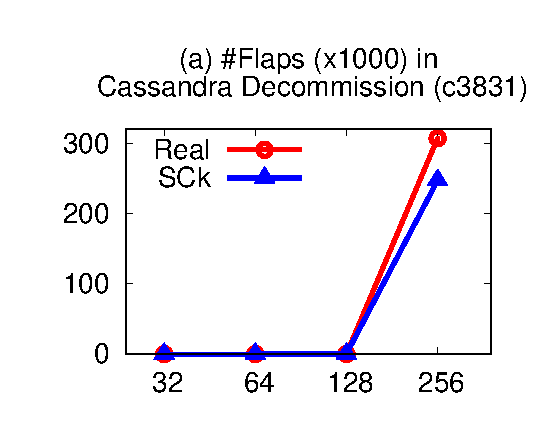
\includegraphics[width=\fgw]{F/old-bugs/eps/cass2.eps}
\hminb
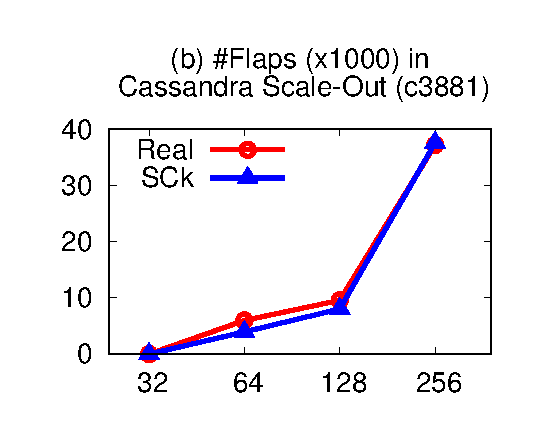
\includegraphics[width=\fgw]{F/old-bugs/eps/cass3.eps}
\hmina
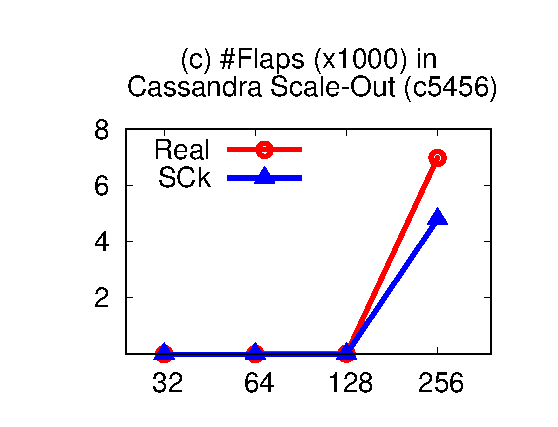
\includegraphics[width=\fgw]{F/old-bugs/eps/cass4.eps}
}
%\centerline{
%\hmina
%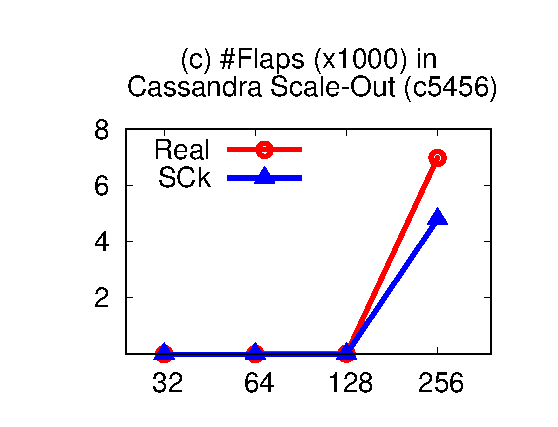
\includegraphics[width=\fgw]{F/old-bugs/eps/cass4.eps}
%\hminb
%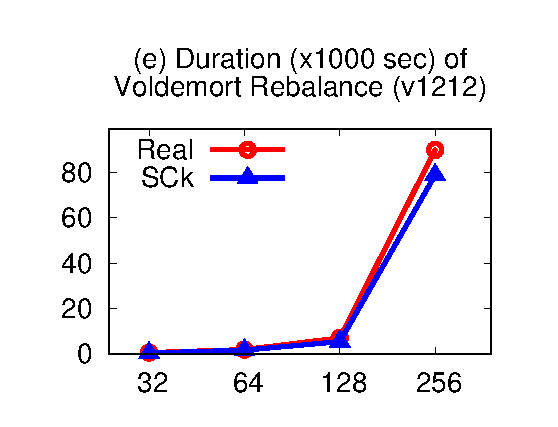
\includegraphics[width=\fgw]{F/old-bugs/eps/vold1.eps}
%}

%\centerline{
%\hmina
%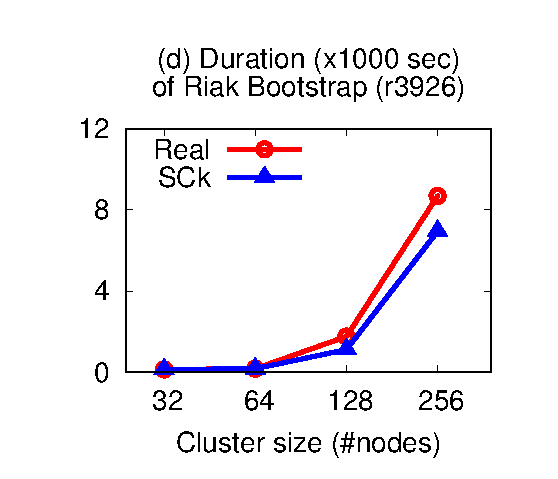
\includegraphics[width=\fgw]{F/old-bugs/eps/riak1.eps}
%\hminb
%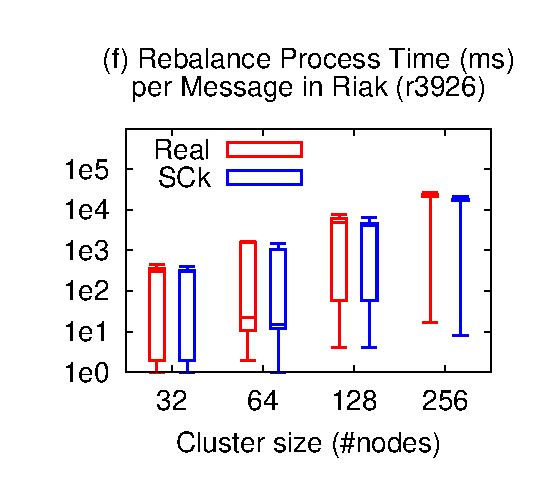
\includegraphics[width=\fgw]{F/riak/eps/proc.eps}
%}

\vminfive

\mycaption{fig-bugs}{Accuracy in reproducing other 
bugs (\sec\ref{eval-bugs})}{The
figures represent the bugs described in Table \ref{tab-bugs}.  
The title represents the y-axis. 
We cap the y-axis to show the scale at which the bug symptoms start
to appear. }
\vminfive
\end{figure}



\if 0

TODO: CASS2: waiting for NOme to go up.
Meanwhile doing CASS3. 
%
RIAK: Buggy done, but need to plug in data from new version
(Cesar is adding fixed/patched line from the newest version).
%
VOLD: (Wait until all features are in).  Still running.
\fi


\subsection{Bugs Reproduced}
\label{eval-bugs}





\begin{table}
\begin{center}
\small
\centering
%---------------------------------
\begin{tabular}{l|r|l|l} 
{\bf Bug\#} & 
{\bf Surface} & 
{\bf Protocol} & {\bf Metric} \\
\hline
\caone \cite{CA-One} &$N$$\geq$256 & Bootstrap & \flaps \\
\catwo \cite{CA-Two}   & $\geq$256 & Decommission & \flaps \\
\catri \cite{CA-Tri}   & $\geq$64 & Add new nodes & \flaps \\
\cafour \cite{CA-Four}  & $\geq$256 & Add new nodes & \flaps \\
\riakone \cite{RIAK-One} & $\geq$128 & Boot+rebalance & $T_{Complete}$ \\
\voldone \cite{VOLD-One} & $\geq$128 & Rebalance & $T_{Complete} $ \\
\end{tabular}
%---------------------------------
\end{center}
\vminten
\mycaption{tab-bugs}{Reproduced bugs (\sec\ref{eval-bugs})}{``Surface'' 
implies the number of nodes
needed for the bug symptom to surface.
``c'' stands for Cassandra, ``r'' for Riak, and ``v'' for
Voldemort. 
}
\vminfive
\end{table}



Table \ref{tab-bugs} lists all the \numEval bugs we  reproduced (4
Cassandra, 1 Riak, and 1 Voldemort, and 4 HDFS bugs).  We chose these
\numEval bugs (among the \totAll bugs we studied) because the reports
contain more detailed descriptions about the bugs, the affected protocols,
the affected code version numbers, configuration setups, and the patches.
%
%Our first target system was Cassandra, hence the more bugs reproduced
%compared to Riak and Voldemort; the latter two were added for  stronger
%proof of concept.
%


Figure \ref{fig-bugs} shows the accuracy of \sck in reproducing the
\numEval bugs using the metrics Table \ref{tab-bugs}.
%
As shown, for Cassandra and Riak bugs where all nodes are CPU intensive
PIL is
needed for accuracy (the \ts{SCk+PIL} vs. \ts{Real} lines 
in Figures \ref{fig-bugs}a-d), 
but for others \stest suffices
(\ts{SCk} vs. \ts{Real} lines in Figures \ref{fig-bugs}e-f).
%
The first bug, \caone, has been described before.
%
We now briefly discuss the other 9 bugs 
and then
%
make several important remarks.


{\bf (a)} Figure \ref{fig-bugs}a: In Cassandra \catwo \cite{CA-Two} when a node D is
decommissioned from a large cluster, all other nodes must own D's
key-partitions.  This scale-dependent ``pending keyrange calculation'' is
CPU intensive, causing cluster-wide flapping (the $y$ axis), observable in
256+ nodes.  The fix caches the outputs of slow methods.


{\bf (b)} Figure \ref{fig-bugs}b: \catri \cite{CA-Tri} is similar to the
previous bug (\catwo), but the fix was obsolete as the concept multiple
key-partitions per node was added.  The calculation is now scale-dependent
to $N$$\times$$P$.  This causes CPU spikes and massive flapping during
scaling out; the bug surfaced in 64+ nodes (when 32+ new nodes are added
to existing 32+ nodes). The bug was fixed with a complete redesign of the
pending keyrange calculation.
%





{\bf (c)} Figure \ref{fig-bugs}c: Interestingly, \cafour \cite{CA-Four} is
a bug in the {\em same} protocol as above.  We found that the previous fix
was obsolete again as pending range calculation is now multi-threaded;
range calculations can happen concurrently.  This new design however
introduces a new coarse-grained lock that can block gossip processing for
a long time, thus introduces flapping (in 256+ nodes).  The fix changed
the lock management.
% The figure also shows that, for this workload, \hsg{profile?} ffline
% time profiling is not fully accurate as the bug is order sensitive at
% large scale.  We are now testing it with order determinism.



{\bf (d)} Figure \ref{fig-bugs}d: In \riakone \cite{RIAK-One}, Riak's
rebalancing algorithm employed 3 complex stages (claim-target, claim-hole,
full-rebalance) that each node runs to converge to a perfectly balanced
ring.  Each node runs this CPU-intensive algorithm on {\em every}
bootstrap gossip received.  The larger the cluster, the longer time the
perfect balance is achieved (a high $y$ value in 128+ nodes).
% This decentralized
% rebalancing was fixed with a centralized rebalancing.  


{\bf (e)} Figure \ref{fig-bugs}e: In \voldone \cite{VOLD-One}, Voldemort's
rebalancing was not optimized for large clusters; it led to more
stealer-donor partition transitions as the cluster size grows (128+
nodes).  The fix changed the stealer-donor partition transition algorithm.


% if no space
%For Riak, we record the rebalancing time along with pre-memoization (with
%order determinism; \sec\ref{sc-pil-3}-\ref{sc-pil-4}).  Figure
%\ref{fig-bugs}f (similar to Figure \ref{fig-accu}d) compares the execution
%time of the rebalance function invocations in \sck and real deployments.
%The figure shows that \sck's PIL exhibits a high accuracy.


% HDFS



% hdfs-9198
{\bf (f)} Figure \ref{fig-bugs}f: In \hdone \cite{HDFS-One}, incremental
block reports (IBRs) from HDFS datanodes to the namenode acquires the
global master lock (\ie, a special worker-to-master ``loop'' as explained
in \sec\ref{sc-find}).  As $N$ grows, more IBR calls acquire the lock.
The IBR requests quickly backlog the namenode's IPC queue; with 256 nodes, the IPC queue
hits the max of 1000 pending requests; $y$=1 ($\times$1000).  When this
happens, user requests are dropped by the namenode.  The fix batches the
IBR request processing.
%
In HDFS, to emulate large blocks, we reuse the ``\ts{TinyDataNode}'' class
(1KB blocks) that the developers already use in the unit tests.


% hd-4????
{\bf (g)} Figure \ref{fig-bugs}g: In \hdtwo \cite{HDFS-Two}, when $D$
datanodes are decommissioned, the blocks must be replicated to the other
$N$$-$$D$ nodes.
%
Every 5 minutes, the \ts{DecommissionMonitor} thread in the namenode
iterates all block/datanode descriptors to check if the $D$ nodes can be
safely decommissioned (its data replication completes).  This thread holds
the global file system lock.  When $N$ is 256+, this process can hold the
lock for more than 10 seconds ($y$$>$$10$), during which user requests
cannot be served.
%
The fix uses a dedicated thread to manage decommissioning and refines the
algorithm.


% hadoop-1073
{\bf (h)} Figure \ref{fig-bugs}h: In \hdtri \cite{HDFS-Tri}, a new file creation, the
namenode calls a \ts{chooseTarget} function to sort a list of target
datanodes from their distances from the writer and choose the best nodes.
When $N$ and the replication factor are large, it can take more than one
second to choose.  The fix patch modifies the sorting algorithm.


% preview F/old-bugs-2/eps/hdfs1.eps
{\bf (i)} Finally, in \hdfour \cite{HDFS-Four} (figure not shown for space),
% Figure \ref{fig-bugs}: HDFS-315 (ongoing) Figure 8?: In hd315 [?], 
datanodes send block reports too frequently and when $N$$>$512 nodes, the
namenode spends more time in this background process as opposed to serving
users.

We make several remarks from this experience.
%
First, \sck can help developers prevent recurring bugs; the series of
Cassandra bugs above involves the same protocols (gossip, rebalance, and
failure detector) and create the same symptom (high \flaps); in other
words, code evolution can re-introduce similar bugs in the same protocols.
%
Second, reproducing scalability bugs is relatively straightforward once we
achieved a high colocation factor.  Unlike non-deterministic bugs which
require complex timing reordering to reproduce \cite{Guo+11-Demeter,
Leesatapornwongsa+14-Samc},
symptoms of scalability bugs are ``deterministically scale-dependent.''
%
%
Third, different systems of the same type (\eg, key-value store) implement
similar protocols.  The  generality of \sck methods in scale-checking
all different protocols above can be useful to many other distributed systems.
%

